\paragraph{Poseidon}

\hspace*{\fill}

\indent \href{https://www.poseidon-hash.info/}{Poseidon} is a hash function designed for the Zero-Knowledge proof system.
Its calculation process is rough as follows:

\begin{figure}[!ht]
    \centering
    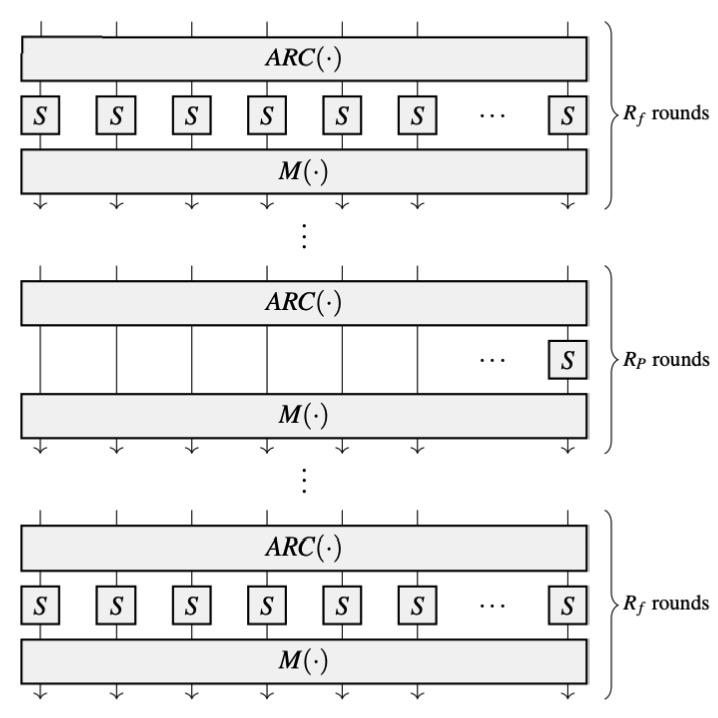
\includegraphics[width=0.6\textwidth]{gates/poseidon_process.jpeg}
    \caption{Construction of poseidon}
    \label{fig:poseidon-process}
\end{figure}

Each round function of Poseidon permutation consists of the following three components.
\begin{enumerate}
    \item ARC(.): AddRoundConstants
    \item S: SubWords
    \item M(.): MixLayer
\end{enumerate}

The Trace of the gate is like this:
\begin{figure}[!ht]
    \centering
    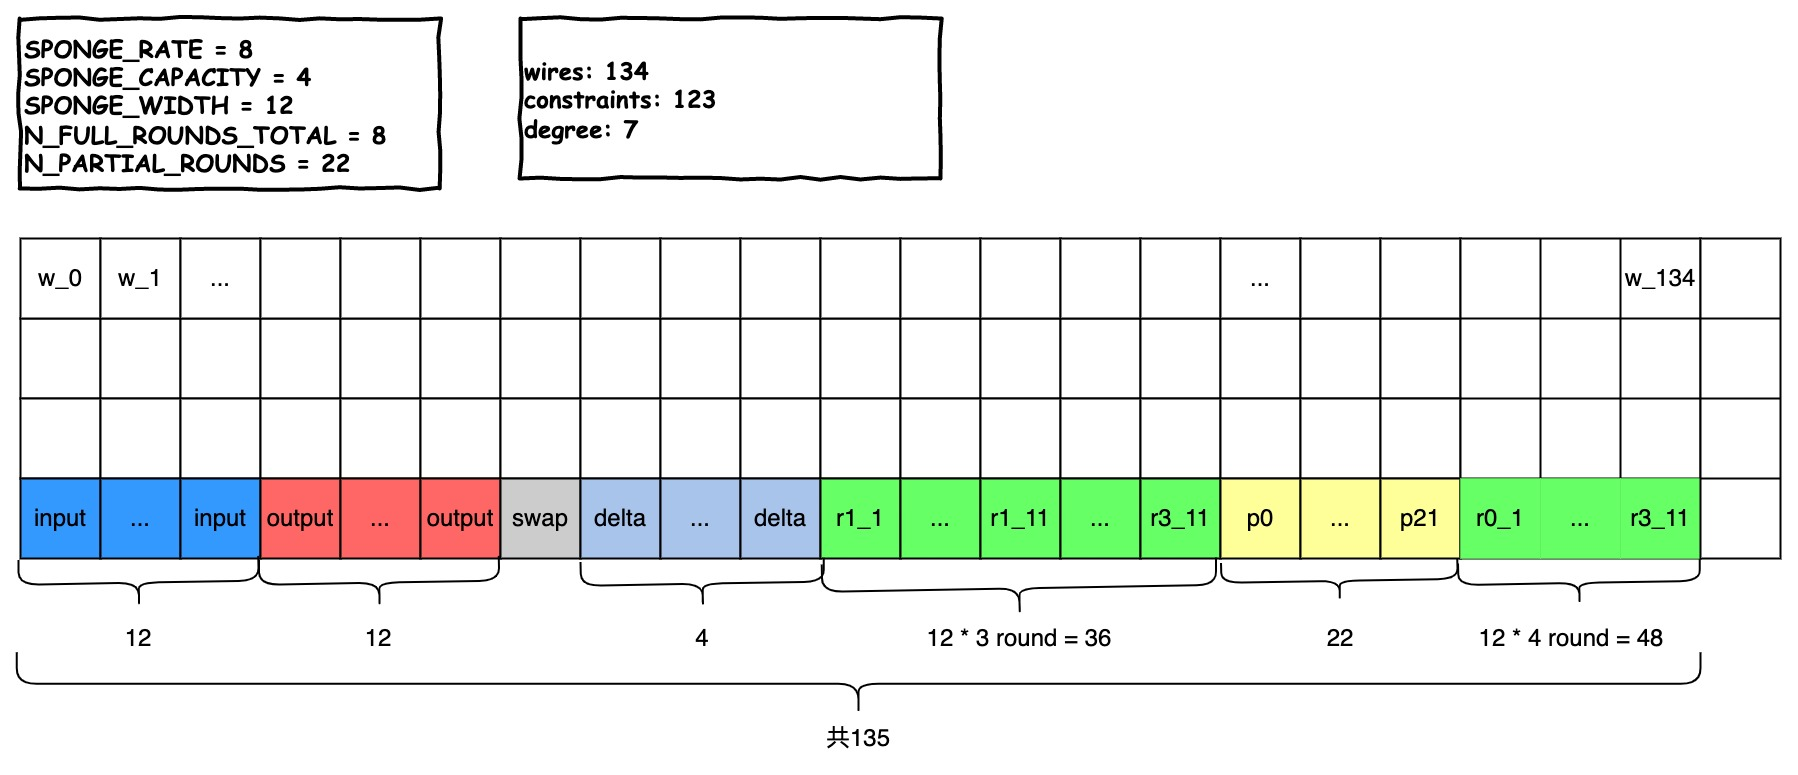
\includegraphics[width=0.6\textwidth]{gates/poseidon.jpeg}
    \caption{PoseidonGate}
    \label{fig:poseidon-gate}
\end{figure}

\begin{itemize}
    \item input: components of the input, 12 elements.
    \item output: components of the output, 12 elements.
    \item swap: 0 or 1, Indicates whether the first four elements of the input are swapped with the last four elements.
    \item delta: used when swap is 1, $\text{delta}_i = \text{swap} \times (\text{input}_{\text{rhs}} - \text{input}_{\text{lhs}})$.
    \item green region: full rounds, ri\_1~ri\_11 is the state of each round.
    \item yellow region: partial rounds, each element is state[0] of each round.
\end{itemize}

Calculation process and related constraints:
\begin{itemize}
    \item Assert that swap is binary. (1 constraint)
    \begin{lstlisting}[language=rust]
constraints.push(swap * (swap - F::Extension::ONE))
    \end{lstlisting}
    \item Assert $\text{delta}_i = \text{swap} \times (\text{rhs} - \text{lhs})$. (4 constraints)
    \begin{lstlisting}[language=rust]
for i in 0..4 {
    ....
    constraints.push(swap * (input_rhs - input_lhs) - delta_i);
}
    \end{lstlisting}
    \item Initialize state: when swap=0, state=input; when swap=1, state is swapped input:
    \begin{figure}[!ht]
        \centering
        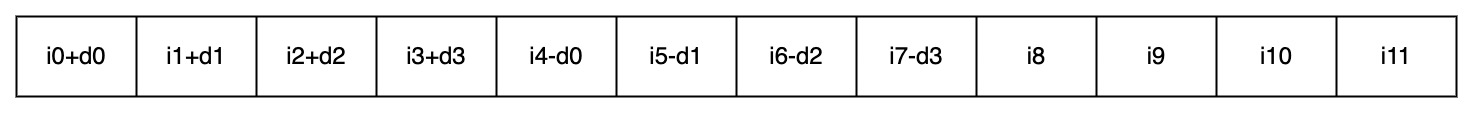
\includegraphics[width=0.6\textwidth]{gates/poseidon_state_init.jpeg}
        \caption{Poseidon State Init}
        \label{fig:poseidon-state-init}
    \end{figure}
    \begin{lstlisting}[language=rust]
for i in 0..4 {
    ...
    state[i] = vars.local_wires[input_lhs] + delta_i;
    state[i + 4] = vars.local_wires[input_rhs] - delta_i;
}
for i in 8..SPONGE_WIDTH {
    state[i] = vars.local_wires[Self::wire_input(i)];
}
    \end{lstlisting}
    \item Begin first full rounds calculation, for each round r (which is 0--3):
    \begin{itemize}
        \item Perform ARC: Add each element of state to the pre-generated value at a particular position in the array.
        \begin{lstlisting}[language=rust]
for i in 0..WIDTH {
    state[i] += F::from_canonical_u64(ALL_ROUND_CONSTANTS[i + WIDTH * round_ctr]);
}
        \end{lstlisting}
        \item Except for r=0, constrain each element of the state calculated in the previous round (the green part of the first slice of the figure). 
        (12 constraints per round, a total of 36 constraints)
        \item Perform SubWords: Turn state element by element x into $x \mapsto x^7$
        \item Perform MixLayer: Each element of the state is updated according to itself and a pre-generated array.
        \begin{lstlisting}[language=rust]
// r is the index of state elements here.
let mut res = F::ZERO;
    for i in 0..WIDTH {
    res += v[(i + r) % WIDTH] * F::from_canonical_u64(Self::MDS_MATRIX_CIRC[i]);
}
res += v[r] * F::from_canonical_u64(Self::MDS_MATRIX_DIAG[r]);
        \end{lstlisting}
    \end{itemize}
    \item Perform partial rounds:
    \begin{itemize}
        \item Perform ARC
        \begin{lstlisting}[language=rust]
for i in 0..12 {
    if i < WIDTH {
        state[i] += F::from_canonical_u64(Self::FAST_PARTIAL_FIRST_ROUND_CONSTANT[i]);
    }
}
        \end{lstlisting}
        \item Processing of state with $11 \times 11$ MDS (maximum distance separable) matrix.
        \begin{lstlisting}[language=rust]
result[0] = state[0];
for r in 1..12 {
    if r < WIDTH {
        for c in 1..12 {
            if c < WIDTH {
                let t = F::from_canonical_u64(
                    Self::FAST_PARTIAL_ROUND_INITIAL_MATRIX[r - 1][c - 1],
                );
                result[c] += state[r] * t;
            }
        }
    }
}
result
        \end{lstlisting}
        \item Perform 22 round sbox, for the first 21 rounds (r = 0--21):
        \begin{itemize}
            \item Take sbox\_in(yellow elements in the figure), and constrains state[0]=sbox\_in -- 21 rounds totally 21 constraints.
            \item \verb|state[0] = state[0]^7|
            \item \verb|state[0] += FAST_PARTIAL_ROUND_CONSTANTS[r]|
            \item Perform mds to state.
        \end{itemize}
        \item For the 22th round:
        \begin{itemize}
            \item \verb|state[0] = sbox_in| (i constraint)
            \item \verb|state[0] = state[0]^7|
            \item Perform mds to state.
        \end{itemize}
    \end{itemize}
    \item Perform second round "Full rounds", same with the first round. (the green part of the second slice of the figure). (12 constraints, 4 rounds totally of 48 constraints)
    \item Asserts computed result equals output. (12 constraints)
    \begin{lstlisting}[language=rust]
for i in 0..SPONGE_WIDTH {
    constraints.push(state[i] - vars.local_wires[Self::wire_output(i)]);
}
    \end{lstlisting}
\end{itemize}

The constraints of this gate in total is 123, the degree is 7 (when performing s-box, making $\text{state}[i] \mapsto \text{state}[i]^7$).
